\chapter{Летописание и летосчисление}

%На время не станем вспоминать, какой нынче год.

В этой книге мы будем обращаться к разным источникам – летописям, хронографам, сагам и так далее. Хронограф это вроде сборника исторических сообщений, куда выписывались сведения из летописей да иностранных хроник. Летописями же принято именовать погодичные перечни событий, относящихся к Руси.

В популярном представлении, летописи велись в монастырях, где за толстыми стенами сидели ученые монахи, из года в год записывая, что происходит вокруг и по соседству, изредка упоминая, какой заморский правитель умер или воцарился. Отчасти это так. Но летописи вобрали в себя сведения из сторонних источников, и являются сборниками. На протяжении веков они подвергались правке с разными целями.

Таковыми могли быть желание дополнить из другого источника, исправить ладность слога, исправить годы, если таковые показались ошибочными, наконец, убрать либо описать другими словами упоминания о некоторых событиях. Ведь издавна существовала цензура, как духовная, так и светская.
 
Листая страницы летописи, мы видим стройную картину. Для каждого года перечислены произошедшие события. Но когда появились в летописи эти даты? Сами ли события эти были записаны под такими годами, или много позже, при последующей правке?

Каждый, кто читает исторические сочинения древних Греков, знает – Греки, сами любители точности и ясного выражения мысли, привязывали события к правлению там-то такого-то царя. Для уточнения могли сказать – в пятый год царствования. Или – в год, когда в Олимпийских играх победил такой-то из указанной страны.

Скандинавы в сагах задают время таким же приемом. Когда там-то правил конунг такой-то, и цепляют повествование за это событие, да за события из других саг, соседних по времени и месту действия, при необходимости прибавляя – «на следующую весну», или «до осени такой-то оставался в гостях там-то, и затем отправился туда-то».

Следы подобного способа счета лет находим и в наших летописях, где не редкость привязка к византийским императорам. Правда, одни и те же события разные летописи иногда относят к разным императорам.

Возникает противоречие. Если летопись А относит крещение княгини Ольги к императору Цимисхию, а летопись Б к императору Константину, значит, в летописях А и Б – разные даты крещения. Какой летописи верить, А или Б? Отложим сей вопрос.

Сохранившиеся до наших дней, известные общественности летописи освещают события разных местностей и городов, с уклоном туда, где происходила правка и дополнение летописи. Во многих летописях первым помещается сочинение «Повесть временных лет» монаха Киевопечерской Лавры Нестора и его последователей, чье содержимое от списка к списку различно.

Самые важные летописи получили в науке названия – Ипатьевская, Лавреньтевская, Никоновская, Радзивилловская – по именам монахов, приложивших руку к их правке и составлению, а также по именам владельцев, например, патриарха Никона и Януша Радзивилла. Когда говорят «Ипатьевская летопись» и «Ипатьевский список», это одно и то же. В свою очередь, с каждого из этих списков сделаны другие списки, тоже с внесением правок.

Летописи известны читателю большей частью по редким выдержкам оттуда в книгах историков и археологов. Выдержки эти даются по изданиям, именуемым Полным Собранием Русских Летописей (знаменитое сокращение ПСРЛ), либо по другим, где наряду с подлинником дается перевод на современный русский язык.

В ПСРЛ летописи предстают перед нами в обработке учеными. Фотокопиями (светописные издания, фотолитографии) тоже издавались, в 1871 году «Повесть временных лет» из состава Ипатского списка, в 1872-м – она же из Лаврентьевской летописи, в 1875-м – Новгородская синодальная летопись, в 1880 – Ремезовская.

Отличия подлинников от обработанных вариантов таковы – нет знаков препинания, пробелы используются выборочно, все буквы одинаковой величины, числа записаны старославянскими буквами, а все буквы тоже воистину «старославянские». Ученые проделывают большой труд по приведению такого текста в удобочитаемый вид. Они меняют буквы на современные, упорядочивают слова в предложения, расставляют знаки препинания, переводят  числа в арабские. Однако, в ходе обработке возможно искажение смысла подлинника.

В известных нам летописях существует несколько основных слоев летосчисления, то есть способов считать годы от определенного опорного события. Опишу эти слои по глубине старины, от древнейшего к новейшему. Поскольку никто раньше меня о таком не писал, не грех и дать слоям имена.

Слой Царский. Это привязка к годам царствования василевсов (императоров) Византии, а также годам правления русских князей.

Слой Росписной. Ключом к пересчету лет из Царского слоя в рамки более широкого отрезка времени служит «роспись годов» – раздел летописи, где последовательно перечисляется, сколько лет прошло от библейского сотворения мира до всемирного Потопа, от Потопа до Авраама, от Авраама до «исхода» Моисея. Такими временными промежутками, или слагаемыми, летописец добирается до Александра Македонского, затем до рождения Иисуса Христа, императоров Византии, а от них к отрезкам правления князей Русских. Сложив эти промежутки, скажем, вплоть до начала княженья Вещего Олега, мы получим год начала правления Олега от сотворения мира. Число лет в каждом слагаемом бывает различно в разных летописях, поэтому слагаемые это не постоянные значения, но переменные.

Слой Годовой. Прямое указание лет, прошедших «от сотворения мира» до события, указанного в летописи. Если в Царском слое написано, скажем, «В царствование Михаила случилось то-то», в Годовом нас ждет простое: «В год такой-то случилось то-то». Казалось бы, даты Годового слоя должны быть вычислены на основе слагаемых из Росписного слоя. Это ведь Росписной слой дает нам временную основу. Однако на проверку, даты Годового слоя зачастую не совпадают с теми, которые можно получить, произведя вычисление со слагаемыми из Росписного слоя.

В летописях присутствуют все три слоя. Однако появились они в списках не одновременно, а последовательно, невесть через сколько лет, по мере необходимости, для упрощения понимания счета лет и привязки к нему событий, а может по иным причинам.

Во время, когда в летопись вводился Годовой слой, летописец, пересчитав в него из Царского слоя годы предшествующих событий, начинал записывать новые события уже в Годовом слое, отказавшись от использования Царского, то бишь опуская привязку к годам правления таких-то императоров или князей.

Сейчас человечество ведет счет лет «от нашей эры», принимая за первый ее год рождение Иисуса Христа. Так стало удобно.

Само понятие года и его составляющих (лет, месяцев, дней) зависит от особенностей календаря – его привязок к перемещению небесных светил и способу учета времени. Раньше календарей было много, да и теперь тоже. Способ считать дни – это календарь\footnote{Французы после своей революции жили по неуклюжему Республиканскому календарю 13 лет в 1792-1805 годах, и менее года в 1871-м. За начало эры считали год провозглашения республики. Недели отменили – вместо ввели «декады» по 10 дней. Но как и в семидневной неделе, выходной был только один. Введение сего календаря вызвало у некоторых небывалое воодушевление – так, в городе Аррасе устроили шествие из 12 групп по 30 человек, олицетворявших дни. Группы были построены по возрасту. В самом конце несли, под балдахином, столетнего старика – добавочный день високосного года. «Старый» новый год, 1 января, запретили. На почтах в этот день вскрывали письма и уничтожали поздравительные. Так вот, поныне даже маститые ученые совершают ошибки при переводе дат из революционного календаря в годы нашей эры. Что же говорить о переводе дат других, более древних календарей?}. А ведение счета дней, годов от определенного опорного события называется эрой.

Таким событием может быть сотворение мира по Библии, основание Рима, Хиджра (переселение пророка Мухаммеда в Медину), начало цикла древних греческих Олимпиад, и так далее.

Например, известна «эра Набонассара», которую использовал астроном Птолемей, положив началом счета лет царствование вавилонского царя Набонассара, в календарной системе Египтян. Птолемей поместил в своем астрономическом труде «Альмагест» таблицу Канон царей (Ассирии, Вавилона, Персов, Македонян, Римлян) с годами их правления, от Набонассара до Антониуса. Некоторые римские хронологи продолжили сей счет, добавляя годы правления римских императоров, по Диоклетиана включительно. После чего начали считать годы уже от Диоклетиана – наступила «эра Диоклетиана».

Каждый промежуток, слагаемое из Росписного слоя летописей – тоже, по сути, маленькая эра. 

В древности Римляне вели счет лет внутри своей эры, Египтяне – своей, Греки – своей, и так далее. Более того, почти в каждом греческом городе-государстве, полисе, действовал свой отдельный календарь. Народы жили по своим календарям и летосчислениям. И события своей истории привязывали к своим календарям и эрам.

Постепенно, народы, обратившиеся в христианство, стали приходить к общему летосчислению, что ныне мы называем «нашей эрой» или «от рождества Христова». Прежде многие тоже пользовались Годовым слоем, но считали годы от сотворения мира. И когда решали перейти на летосчисление от рождества Христова, надо было всего-то определить, в каком году «от сотворения мира» родился Христос, и потом уже вычислять год по-новому.

К примеру, выдуманный мною народ Буквоедов полагал, что Христос родился на 100-м году от сотворения мира. Стало быть, если в старинной летописи Буквоедов событие «Был неурожай капусты» подписано годом 250-м от сотворения мира, то надо от летописного года отнять год рождения Христа (тоже из расчета от сотворения мира), то бишь 250-100=150. Таким образом 250-й год от сотворения мира это 150-й год от рождества Христова, или 150-й год нашей эры.

Замечательно!

Но вот другой народ, Медоквасы, полагали, что мир был сотворен за 300 лет назад от рождения Христа. И когда в летописи Медоквасы писали «в году 250 от сотворения мира царь Горох построил город Пирогов», мы, чтобы перевести эту дату в современную, должны от 250 отнять 300. Получаем минус 50, то бишь 50-й год до рождества Христова, до нашей эры.

В пределах летописи Медоквасов всё в порядке. В пределах летописи Буквоедов – тоже. Все пишут даты от своего сотворения мира, все счастливы.

Но вот Буквоеды через несколько веков решили расширить свою летопись, да вписали в нее события из летописи Медоквасов, вместе с датами, как есть, ничего не пересчитывая. У Буквоедов в летописи теперь получается:

\begin{quotation}
Год 250. Был неурожай капусты. А у Медоквасов в царстве построен город Пирогов.
\end{quotation}

А ведь даты от сотворения мира у Медоквасов и Буквоедов разные! Но в новом варианте летописи Буквоедов это не учтено. Спустя много столетий ученые начинают переводить даты летописи Буквоедов из счисления «от сотворения мира» в «от нашей эры», или «от рождества Христова». Берут, конечно же, формулу, применимую к Буквоедам. 250-100=150. В ученых книгах появляются строки выдержки из летописи, выглядят уже так:

\begin{quotation}
Год 150 (250 от сотворения мира). Был неурожай капусты. В царстве Медоквасов построен город Пирогов.
\end{quotation}

В других ученых книгах, последующих, того короче:

\begin{quotation}
В 150 году нашей эры медоквасы построили город Пирогов.
\end{quotation}

Таким образом чисто летописно, событие построения города Пирогова было смещено во времени.

Сей упрощенный пример целиком относится ко всем летописям, хроникам, хронографам, короче говоря давним источникам. И мы скоро столкнемся с тем, что применение иной, нежели общепринятая, формулы пересчета лет – более правдоподобно. И с тем, какая путаница среди дат есть в летописях, о чем историки предпочитают молчать, используя в своих работах только общепринятые списки, но и там при вдумчивой проверке вскрываются странности.

Среди летосчислений, основанных на Библии, не было единогласия по поводу того, когда же был сотворен мир. Если сказать это другими словами – в разных эрах год рождения Христа отдален от сотворения мира на разное количество лет. Посмотрим, на какой год «от сотворения мира» приходится рождение Христа в вариантах летосчисления:\\

\noindent
Александрийская эра: 5492\\
Византийская эра: 5508-5509\\
Византийские хронисты Максим Исповедник, Феофан Исповедник и Георгий Синкелл: 5493\\
70 толковников: 5508\\
Самаритянский текст: 4700\\
Римские хронографы: 3948\\
Иудейская эра: 3761\\

%\begin{table}[h]
%\begin{tabular}{|l|l}
%\hline
%Александрийская эра & 5492\\ \hline
%Византийская эра & 5508-5509\\ \hline
%Византийские хронисты Максим Исповедник,\\ Феофан Исповедник, Георгий Синкелл & 5493\\ \hline
%70 толковников & 5508\\ \hline
%Самаритянский текст & 4700\\ \hline
%Римские хронографы & 3948\\ \hline
%Иудейская эра & 3761\\ \hline
%\end{tabular}
%\end{table}

Есть множество других.

С некоторых пор на Руси пользовались счислением, принятым в «Византийской эре». Затем, на ее 7208 году, Петр I указом ввел счисление «от рождества Христова». Так год 7208 стал годом 1700. Другие страны переходили на новую эры кто раньше, что позже.

Ученые пишут, что Византийский счет годам использовался на Руси со времени крещения князя Владимира Красна Солнышка. Подобное мнение успокаивает, придает летописным датам весомость, и облегчает пересчет летописного, от сотворения мира, года в «нашу эру», от рождества Христова.

Наука история использует для этого следующие правила.

Общее, упрощенное – от летописного года отнять 5508. Например, 6360-5508=852. Однако это правило требует некоторых уточнений.

До петровского преобразования летосчисления, было два «календарных стиля» – мартовский (пришел к нам из Рима) и сентябрьский (византийский). По первому, началом года считали март, по второму – сентябрь. Неясно, когда мартовский сменился сентябрьским. Полагают, что в конце 15 века.

Для мартовского календарного стиля правило пересчета уточняется. Если у нас есть летописная дата с указанным месяцем, и месяц этот – начиная с марта и по декабрь включительно, надо от летописного года отнять 5508. Если же месяц – январь или февраль, мы отнимаем от летописного года число 5507.

Теперь уточнение для сентябрьского календарного стиля. Ежели месяц с января по август включительно, от летописного года отнимаем 5508. Если месяц – с сентября по декабрь включительно, то отнимаем 5509.

Какие стили в каких источниках использовались? А это вечная пища для ума историков. В той же «Повести временных лет» будто есть оба стиля. Погрешность в датах, при переводе, плюс-минус один год, и так во многих древнерусских источниках.

Одним словом, формулы выработаны. Как здорово! Значит, любой год из летописи можно перевести в «нашу эру»! Но верно ли полагают ученые?

Прежде чем вести разговор дальше, я должен поведать еще об одном слое датировок. Я нарочно вынес его отдельно, чтобы не определять его положение между другими слоями.

Слой Индиктов.

Рим собирал с каждого побежденного народа дань трижды за 15 лет. На пятнадцатом году император объявлял размер дани на следующие пятнадцать лет. Латинское слово «indiction» значит «объявление», потому и год нового объявления податей назывался индиктом. Более ходовое значение слова «индикт» – просто такой-то год внутри пятнадцатилетнего цикла. Сами циклы никак не нумеровались.

В старинных источниках, в том числе наших летописях, встречаются датировки по индикту. Например, если написано, что событие случилось при Михаиле царе, в индикт 12, это значит 12-й год одной из пятнадцатилеток во время правления Михаила. Какой именно пятнадцатилетки – остается неясным.
 
Теперь, вооружившись знаниями, попробуем разобраться с датами в русских летописях и сравним наши исследования с тем, что предлагают ученые – а предложенное ими составляет основы исторической науки.

Откроем Ипатьевский список, время создания коего относят к концу 14, началу 15 веков. Издание 1871 года, подготовленный учеными текст. Летописец начинает рассказывать, в каком году, по его, летописца, источникам, стала впервые прослеживаться «Руская земля», то есть когда впервые ее упомянули. Избранная мною выдержка не случайна, в ней используются все четыре слоя летосчисления – Царский, Росписной, Годовой, Индиктов:

\begin{quotation}
В лето 6360, индикта 15, наченшю Михаилу царьствовати\footnote{Речь идет о византийском императоре Михаиле.}, нача ся прозывати Руская земля. О сем бо уведахом, яко при сем цари приходиша Русь на Царьград, яко же пишет в летописании Грецком\footnote{Об этом узнаём, поскольку при сем царе Русь приходила войной на Царьград, как сказано в летописании Византии.}; тем же и отселе почнем и числа положим:

яко от Адама до потопа лет 2242; а от потопа до Аврама лет 1082; от Аврама до исхождения Моисеева лет 430; от исхождения Моисеева до Давида лет 601; от Давида и от начала царства Соломоня до пленения Иерусалимова лет 448; от пленения до Александра\footnote{Македонского.} лет 318; от Александра до Христова Рождества лет 333; от Христова Рожьства до Костянтина лет 318; от Костянтина же до Михаила сего лет 542.

От первого лета Михаила сего до первого лета Олгова\footnote{Вещего Олега.}, Рускаго князя, лет 29; от первого лета Олгова, понележе седе в Киеве, до первого лета Игорева 31; от первого лета Игорева до перваго лета Святославля лет 33; от перваго лета Святославля до перваго лета Ярополча лет 28; Ярополк княжи лет 8; Володимер княжи лет 37. Ярослав княжи лет 40. Темьже от смерти Святославля до смерти Ярославли лет 85; от смерти Ярославли до смерти Ярополчи лет 60.
\end{quotation}

Что же? Переведем в «нашу эру», «от рождества Христова» дату 6360 «от сотворения мира» из Годового слоя так, как делает наука. От летописного года отнимаем 5508. 6360–5508=852 год нашей эры. Это число находим в учебниках, его же ученые используют в своих трудах.

Давайте проверим знаменитую формулу, по которой ученые перекладывают летописный год в нашу эру. А они говорят, что в летописи принято, будто Христос родился на 5508 году после сотворения мира.

Но вот перед нами, выше, выдержка из научного, однако не фотографического, издания списка Повести временных лет. Используя числа из его Росписного слоя, подсчитаем, сколько лет прошло от Адама до рождения Христа.\\

2242+1082+430+601+448+318+333=5454\\

5454! Простите, 5454 равно 5508? Нет. 

Так сколько лет отнять от летописного года? То, что говорят ученые, или что сказано в летописи? Разница в 54 года.

Однако проверим саму Ипатьевскую летопись печатного издания ПСРЛ. В ее Годовом слое написано, что Михаил начал царствовать в 6360 году.

По данным Росписного слоя этой же летописи, сколько лет прошло от сотворения мира до начала правления Михаила?\\

5454+318+542=6314\\

Разве 6314 равно 6360? Нет. 

Значит, закралась ошибка. Где именно? В дате Годового слоя или в слагаемых Росписного? Даты Годового слоя, кажется, должны вычисляться по числовым значениям из Росписного, и может быть, что при вычислении «года от сотворения мира» правщик летописи просто ошибся, складывая числа.

Закроем глаза на Годовой слой. 

Используя Росписной слой, вычислим, когда «нача прозывати Руская земля». Летопись привязывает это событие к началу царствования Михаила. Оно, по данным Росписного слоя, приходится на 6314 год от сотворения мира. Пересчитаем 6314 год в эру «от рождества Христова», продолжая работать с числами из Росписного слоя:\\ 

6314-5454=860 год от рождества Христова.\\

Таким образом, по Годовому слою и ученой формуле, 852 год от рождества Христова, а по данным из Росписного слоя – 860 год от рождества Христова.

Если же предположить, что число из Годового слоя 6360 всё же вернее, но год рождения Христа взять из Росписного, а не из представлений ученых, то бишь использовать 5454 вместо 5508, вычисление будет следующим:\\

6360-5454=906 год от рождества Христова.\\

Даже на таком простейшем уровне проверки летописных данных возникает путаница, и не знаешь, каким числам доверять.

Вы скажете – всего делов! Взять и поглядеть в энциклопедии, когда в Константинополе правил император Михаил! Но ведь и энциклопедическая дата – вычислена. А вычислять, как видим, можно по-разному.

Берем другой весомейший список, Лаврентьевский, в изданиях серии ПСРЛ. Он пожалуй самый древний среди известных, ибо оснащен припиской на обороте 172 листа, что списан мнихом Лаврентием в Суздали для великого князя Дмитрия Константиновича в... Но каком году? Ученые говорят, что в 1377-м. 

Но это трактовка! В подлиннике стоит – в лето «6 800 80 5». Это я переложил старославянские цифры в арабские. Получается 6885 год от сотворения мира. Так написал монах Лаврентий. А по научной формуле, какой это будет год от рождества Христова? 6885-5508=1377.

«Слагаемые» истории в Росписном слое этого издания Лаврентьевской летописи немного отличны от Ипатьевской летописи, однако отличия начинаются после Вещего Олега и они незначительны, в пределах трех лет.

Но вчитаемся в примечания, коими снабжена летопись. Оказывается, ученые, подготавливая список к печати, исправили многие «слагаемые», приведя их в соответствие с данными из других списков!

Давайте поглядим в подлинник. 

\begin{center}
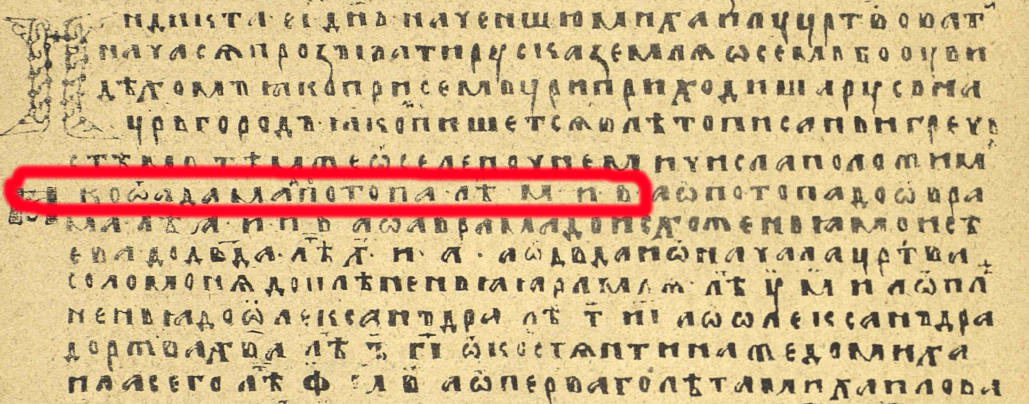
\includegraphics[width=\linewidth]{chast-colebanie-osnov/letois/lavr-sveto-01.jpg}
\end{center}

В светописное издание Лаврентьевской летописи, страницу 12. Промежуток лет от Адама до потопа задан так: «яко от адама до потопа лет 40 и 2», цифры обозначены буквами М и В.

Это 42.

А в обработанном издании? Там указано число 2242.

Разница между подлинником и обработанным текстом – 2200 лет.

Что это значит? Много чего! Выходит, в Лаврентьевском списке, даты вовсе не по счету Византийской эры. Временная шкала, используемая в Лаврентьевском списке, сдвигается на 2200 лет – при проверке первого же «слагаемого» из Росписного слоя в подлиннике! А значит, Иисус рождается на 2200 лет от сотворения мира раньше – по эре, используемой в Лаврентьевской летописи.

Я не изучал еще на этот счет светописные издания других летописей, кроме Лаврентьевской, но полагаю, что в подлинниках откроется много любопытного касаемо используемых эр и датировок.

Что же ученые? Проводят ли они нехитрые вычисления, доступные любому школьнику, чтобы определить, какое летосчисление применено в каждой отдельной летописи?

Нет. Они просто берут данные из Годового слоя, да еще обработанного правщиками изданий ПСРЛ, и по заученной формуле переводят числа из одной эры в другую. С данными из подлинников, а также с данными из Росписного слоя никто не работает.

Существует довольно мало книг о хронологии русских летописей, в эти мутные воды редко кто решается войти. Да и, мало кому приходит в голову выяснять, как же летописец считал годы, каким способом.

Одна из основных работ на эту тему, «Хронология русского летописания» Николая Георгиевича Бережкова, вышла в 1963 году смешным по тем временам тиражом – 1600 экземпляров. Это указывает еще и на степень востребованности историками подобных трудов. Бережков занимался вопросом, положенным им в название книги, с 1939 года.

Выявлены ли в «Хронологии русского летописания» слои летосчисления? Нет. Соответственно, не проведена проверка данных из этих слоев на соответствие друг другу. Какие числовые данные использованы в книге? Из обработанных изданий летописей. А мы знаем, что в подлинниках числа оказываются другими.

И здание науки стоит на зыбучем песке.

На всех страницах Бережков предполагает, что счет лет во всех рассматриваемых им летописях отличается только по годовому стилю – сентябрьскому, мартовскому и ультрамартовскому. И все вычисления крутятся около числа 5508.

Веками длится правка чисел в летописях. Веками же ученые используют эти правленные-переправленные числа, даже не помышляя о проверке, о том, чтобы определить, как даты появлялись в летописях.

Первое привело к тому, что у нас нет никаких четких датировок давних летописных событий. Второе – что мы используем ошибочные датировки всех событий вообще, включая современные, потому что числовое значение года рождения Христа, определенное в рамках «нашей эры» – тоже вычислено на основании чисел, взятых в мешанине различных летосчислений.

Казалось бы, современная наука отошла от религии, и ученые изучают следы явлений, произошедших, как полагают, за миллионы лет до нашей эры. Находят, допустим, скелеты динозавров, и говорят – динозавры жили 200 миллионов лет назад. Или 100 миллионов. И те же ученые, не моргнув глазом, используют временную шкалу, основанную на сведениях Библии о сотворении мира в предшествующие нам 10 тысяч лет. Так что это, вера или наука? Или наука и есть вера?

В моей ненаучной книге я вынужден делать много оговорок об использовании данных из разных источников. Как использую, почему, и указывать степень своего доверия к приводимым сведениям. Увы, я не имел сил и рвения затеять сверку всех чисел из доступных мне светописных копий – сверку как между копиями, так и с «подготовленными» учеными текстам в изданиях ПСРЛ. Делал это отрывочно и по мере надобности, а должно быть у общей картины выявил бы любопытные закономерности, или вообще запутался.

В целом для цитат, если не разбираю нечто крайне важное, я обращаюсь к «подготовленному» изданию 1908 года Ипатьевского списка, да изданию 1926-1928 Лавреньевского, это из имеющихся у меня изданий лучшие, кроме светописных.

А что мне делать с датами? Датам из каких списков отдавать предпочтение? Из какого слоя какой летописи? Нет у меня ответа, и вынужден я пользоваться датами общепринятыми, порицая оные и указывая на их шаткость.

Некоторые летописи содержат дополнительные сказания, такие как «Сказание о Словене и Русе и городе Словенске», где читаем:

\begin{quotation}
И в лето от сотворения света 3099 Словен и Рус с роды своими отлучишася от Ексинопонта, и идоша от роду своего и от братия своея.
\end{quotation}

Потирая руки, применяем известную формулу в общем ее виде. От летописного года отнимаем год 5508:\\

3099-5508=-2409\\

Это же 2409 год до нашей эры! Здесь одни ученые говорят – не может быть, выдумка новгородских книжников. А другие находят подтверждение следов древнейшей истории Славян.

Но разве мы знаем, какое летосчисление использовалось в «Сказании»? Давайте-ка на пробу применим к нему летосчисление не Византийской эры, а другое. Например, из римских хронографов. У них сотворение мира отнесено к 3948 году до нашей эры. Давайте подсчитаем. От летописного года 3099 отнимем 3948. Получим 849 год до нашей эры. Тоже звучит фантастически, но всё же в меньшей степени, чем третье тысячелетие до нашей эры.

Может быть, в истинном летосчислении «Сказания», число 3099 при переводе на «от рождества Христова», относилось бы, скажем, к девятому веку нашей эры.

Время и место. Так называется замечательный роман Юрия Трифонова, однако от времени и места зависит счет лет. Из-за того, что в летописи попали сведения из разрозненных источников, зачастую трудно сказать, насколько верна эта дата по отношению к Годовому слою летописи-приемника. И чем глубже в историю, тем более летописные даты теряют основательность.

А какое было летосчисление до принятия Владимиром христианства\footnote{Читатель, да услышь ехидство в сем вопросе!}? Повесть временных лет охватывает часть времен поганских. Нестор не был им свидетелем и пользовался чужими рассказами. Надо полагать, в этих его источниках существовали свои летосчисления. Какие? Загадка.

Но хорошо.

Мы сейчас ведет счет лет «от нашей эры», то бишь от рождества Христова. Привычно и понятно.

Но ведь разные народы в разное время перешли на такое летосчисление. Однако положим, кто-то раньше других. Сейчас мы, после цепочки произведенных во глубине веков вычислений, пользуемся годом рождения Христа, вычисленным монахом Дионисием Малым\footnote{Скиф Дионисий слыл образованнейшим духовным лицом Рима во времена папы Иоанна I. В математических расчетах Дионисий использовал ноль, чего среди его современников не водилось.}. Дионисий при вычислениях считал годы по современной ему Диоклетианской эре. Ею пользовались христиане Египетской Александрийской церкви, а ныне Коптская православная церковь. Вопрос, насколько верно вычисление Дионисия, оставим в стороне. Эру же «от рождества Христова» впервые ввел в обиход – в своих научных трудах – другой монах, Бэда (Beda Venerabilis).

Когда в какой-то стране возникала надобность перейти на эру «от рождества Христова», то соотносили рождество Христово в счете лет Диоклетианской эры с годом рождества Христова по местному летосчислению. Но мы уже видели на примере русских летописей, что год рождения Христа в них, в зависимости от списка, легко прыгает на тысячу лет. События могут смещаться – в письменной истории – на тысячу лет относительно рождества Христова, нашей эры. 

Поскольку приняли полагать, что числа в одних летописях верны, а в других ошибочны, то в основе датировки событий лежит вера. Вера в определенную летопись.

А когда начали вести счет годам от рождения Христа? С дня его рождения? Нет. Сразу после его смерти? Тоже нет. Когда же?

Столетия спустя.

Как вообще можно узнать, когда родился Иисус?  Выясним, какие временные привязки существуют у этого события.

В Библии не написано, что в таком-то году от сотворения мира. Но вроде бы есть много способов  вычислить год рождения\footnote{Способ с привлечением царя Ирода не прокатит – наместников Иудеи под таким именем было 9 – целая династия, и все Ироды.}. Например, известно, что судили Иисуса при Понтии Пилате (Pontius Pilatus), пятом по счету римском управителе провинции Иудеи. Историческое лицо. Когда он родился? 

Единственные, по большому счету, известные упоминания о нем в давних источниках, помимо Нового Завета, находим у римских историков Тацита и Флавия Иосифа. Тацит просто сообщает в своих «Анналах», что Христа казнил «при Тиберии прокуратор Понтий Пилат». Флавий Иосиф перечисляет римских наместников Иудеи, среди них Пилата. Понятное дело, что оба историка в лучших традициях своего времени не используют даты, но делают отсылки к правлению императоров.

А даты их правления, худо-бедно, с некоторых пор появляются в истории, причем поначалу в летосчислении «местных» эр.

На каком-то этапе развития человечества, возникла необходимость эти местные летосчисления соотнести между собой. И каждый ученый, светский или церковный, делал по-своему. А многие не делали, ибо трудно до невозможности. Ведь надо увязать не просто летосчисления, но и календари.

До революции 1917 года, у нас использовался юлианский календарь – его счет дней года известен как «старый стиль», а год начинался с марта (потом начало года перенесли на сентябрь). Имя своё календарь получил от Юлия Цезаря, при коем был введен в обиход.

Сейчас мы используем григорианский календарь. Разница между днями обоих календарей медленно растет – поначалу это было 10 дней, в 1900-2100 годах составляет 13 дней, потом увеличится до 14, а с 2200 года до 15. Поэтому наш странный праздник «старый Новый год» приходится на григорианское 13 января, что по юлианскому календарю – 31 декабря. Ибо от 13 января отнимаем разницу счета дней в этих календарях, равную 13.

Французский ученый Жозеф Скалигер (Joseph Justus Scali\-ger, 1540-1609) ввёл в обиход искусственную эру – ее называют теперь эрой Скалигера или юлианским периодом. За начало этой эры, в рамках юлианского календаря (системы счета дней), Скалигер положил (в пересчете на современную нам эру) 4713 год до нашей эры. Число взято не с потолка, а является произведением множителей 28*18*15, имеющих важные календарные и астрономические значения.

Скалигер в своих работах «Сочинении об исправлении хронологии» и «Сокровищнице хронологии» предложил таблицы перевода дат из различных эр в «свою», таким образом ученые получили в руки средство преобразования дат в привычные, переводя сначала дату в эру Скалигера, а затем из эры Скалигера – в нашу, основание которой тоже вычислено цепочкой таблиц и формул. 

Любое звено этой цепочки может быть ошибочно.

В эре Скалигера все дни (в смысле дня, определяемом юлианским календарем) последовательно нумеруются. Ученые берут какую-нибудь другую эру, например Набонассара, и вычисляют, на какой по счету день эры Скалигера приходится первый день эры Набонассара. Теперь даты, выраженные в счете лет Набонассара, можно соотносить с эрой Скалигера, а через нее – с нашей эрой.

Таким образом, подобные вычисления основаны на пользовании таблицами Скалигера. Быть может, он предлагает алгоритм, способ, по которому сам получил значения в таблицах? Допустим, зная правила умножения, мы можем составить таблицу умножения. А какие правила использовал Скалигер для своих таблиц? Он не пишет. А ведь хорошо бы знать, чтобы проверить!

Последователем Скалигера, в 17 веке, был тоже француз, иезуитский теолог Дионисий Петавиус. В своих трудах по хронологии он выстроил картину истории мира, расположив события по годам, используя как опорные события библейское сотворение мира и рождество Христово. Например, согласно Петавиусу, всемирный потоп случился на 1656 году от сотворения мира, и в 2329 году до рождества Христова.

Сравним с данными «удобочитаемого» издания Ипатьевской летописи. Потоп – 2242 год от сотворения мира, и 3212 лет до рождества Христова.

Петавиус давал также годы по эре Скалигера. Основные сочинения Петавиуса в области хронологии –  «Opus de doctrina temporum» и «Rationarium Temporum» – непревзойденные по охвату событий труды, где расписывается история человечества от сотворения мира и до времени самого Петавиуса. Упорядочение всего по годам! Какая адова работа проделана!

В веках, которые мы знаем как 15-17, ученые Европы принялись разбираться в летосчислениях разных народов, пытались сопоставлять. Год рождения Христа вроде бы уже имели, однако с привязкой – от основания Рима, что порождало несколько вариантов.

Скалигер, как показалось, внес некоторую ясность и предложил способ соотносить эры, упорядочивая историю. По Скалигеру, мир был сотворен за 3949 лет до рождения Христа.

Петавиус, продолживший дело Скалигера, применил его таблицы, разложив по ним события мировой истории. Петавиус внес также исправления. Он полагал, будто Иисус родился за 3984 года после сотворения мира. Начало эры Скалигера (Юлианского периода) имеет привязку – 764-й год до сотворения мира. Сдвиг Петавиусом времени сотворения мира означал «исправление» начала Юлианского периода – Петавиус соотнес его с 729 годом до сотворения мира.

Наконец, Джеймс Ашер в 17 веке поместил сотворение мира на расстояние 4003 лет до рождения Христа, и начало Юлианского периода связал с 710 годом до сотворения мира. Подобных чисел держался и другой ученый того времени, Джон Лайтфут.

Вооруженные таблицами и работами друг друга, христианские ученые-хронологи честно трудились над упорядочением истории, то бишь расставляя по годам события, описанные в разных источниках. Расставляя по годам «от сотворения мира» и от «рождества Христова», невзирая на то, что представления об этом у разных ученых были разные.

Но постепенно все стали приходить к некоему согласию. А оторванные, лежащие где-то в прошлом военные походы Александра Македонского, большой пожар в Риме при императоре Нероне, интриги византийского двора при Цимисхии, и даже вечно враждующие ярлы и бонды из скандинавских саг обрели четкую прописку в истории, получив свои года.

Сейчас у нас некоторый год, скажем, 2015 или 2200.  Я не знаю, когда вы читаете эти строки. Находясь, допустим, в 2066 году мы можем двигаться по одному году назад, и читая документы за эти годы, выяснять историю определенной страны. Время, для которого и ниже которого документы заканчиваются – хронологическая муть. Датировки событий, относящиеся к ней, вычислены. А мы видим, какая невероятная путаница лежит в основе этих вычислений.

Посему год 2022, или год 2200 – не более чем удобная условность для счета лет. 2022 на деле может не означать, что Христос родился 2022 лет назад. Мы не «досчитаем» назад до рождения Христа, у нас нет непрерывной цепочки датированных документов, тянущейся к этому событию. Таким же образом год допустим 860-й, приуроченный к чему-то в учебнике, может не означать, что такое-то событие случилось в 860 году нашей эры.

Далее в этой книге, конечно же, будут встречаться даты. Я согласен с относительной верностью дат, события которых записаны в то же время. Например, знаменитый краевед Киева Николай Закревский родился в 1805 году. И в какой-нибудь церковной книге был записан день его рождения. Тот год современники считали 1805-м.

Летописные годы из Повести временных лет, вплоть до Владимира, Ярослава и пожалуй несколько далее – как к ним относиться? Там же разнобой в списках! Что мне, все варианты перечислять? И каждый переводить в «нашу эру»? А на основании какого слоя – Царей, Росписного или Годового? А может Индиктов?

Ученым проще – они взяли книжку коллеги или предшественника, там готовые числа, и никаких вариантов. Верь им, бери да используй! А я не знаю, какие числа правильные. Я как мог дошел вниз, к доступному мне основанию, и не знаю, каким числам доверять, каким нет.

Поэтому я решил так. Даты буду приводить как в Годовом слое источников, принимая за таковые обработанные тексты из Полного Собрания Русских Летописей. Да и что толку даже от подлинников, если в них разные летосчисления и даты? Разные!

На вопрос, какое же летосчисление верное, и как по годам «нашей эры» разложить летописи разных народов, предания, саги, я отвечу просто – никак. Отсутствие четкой основы современного летосчисления. Слабая взаимосвязь давних источников. Разнобой летосчислений и числовых значений в пределах даже источников одного вида (например русских летописей).

Можно перебросить мостки между некоторыми летописями и сагами. У нас Ярослав, у них – Ярицлейв. Но это уровень слоя Царей. Правы были Греки, что не заморачивались и применяли в своих сочинениях этот слой!

Благодаря путанице дат, если не доверять научной хронологии, то вполне можно предположить – однако ни проверить, ни опровергнуть – что, допустим, поход аргонавтов за Золотым Руном происходил во времена князя Кия. Ведь нельзя же четко сказать, когда ходили за Золотым Руном, хотя историки относят сие событие, подробно описанное Греками, к сказкам.

Кстати о сказках. Прошлое многих народов уходит корнями в то, что ученые именуют мифом, легендой.

Про былое Киева сложно говорить, оно до Кия словно отрезано. А вот возьмем историю Ирландии. Ее исторические предания наука делит на сказочные и настоящие. Хотя в самих преданиях такого разделения нет. Существует список правителей Ирландии – и тоже, одних правителей ученые называют настоящими, других – легендарными! А почему?

В старейших известных временах Ирландии, люди – лишь одни из действующих лиц. В подробно описанной череде событий действуют представители множества народов, среди них основные – Фир Болг (Фирболг), Фомойры, Туаха Дэ Дананн (Tuatha De Danann, что обычно, полагаю ошибочно, переводят как «Народы богини Дану») и клан Мила, да вот только... К простым людям относятся определенно лишь представители клана Мила.

Прежде враждовавшие, Туаха Дэ Дананн и Фомойры потом смешались. Позже Ирландию завоевывали люди, а именно «сыновья Мила» или «клан Мила» – Скифы-выходцы из Египта, прибывшие через Испанию. Затем Туаха Дэ Дананн совершили странный исход с лица земли. Его смысл ускользает из преданий, но сходен с исходом сказочного народа «чуди белоглазой». После своего сокрытия, представители Туаха Дэ Дананн постепенно прослыли эльфами или фэйри, чудесным народом.

%проявляют те же свойства, что эльфы, однако я не уверен, что полное отождествление будет точным, хотя среди исследователей этого вопроса прижилось считать народы богини Дану эльфами.

Я понимаю, сразу перед глазами встает остроухий образ из фантастических произведений, однако нет никаких указаний на необычность внешности Туаха Дэ Дананн, в отличие от Фомойров. Туаха Дэ Дананн, однако, обладали некими способностями, которые люди именовали волшебными.

Так вот, известно 142 правителя Ирландии, которых ученые относят к выдуманным. Известны годы их правления, составлены генеалогические деревья, кто чей сын, дочь или брат, но вот беда, такой-то правитель – из Туаха Дэ Дананн или Фомойров.

Для примера, и сравнения с нашими летописями, приведу выдержку из одной ирландской летописи – Анналов королевства Ирландии (Annála Ríoghachta Éireann). Их составили в 17 веке, пользуясь разными источниками, ученые монахи ордена францисканцев. Их кстати не беспокоило, что речь в значительной части Анналов идет про «волшебные» народы.

Вот мой перевод самого начала этой ирландской летописи, выполненный с английского перевода 1856 года (семитомник Annals of The Kingdom Of Ireland by the four masters)\cite{annals4mast}. Повествуется о начале заселения Ирландии. Имена оставляю в английском написании:

\begin{quotation}
От сотворения мира до года Потопа, 2242 лет. Сорок дней до Потопа, Ceasair\footnote{В анналах Clonmacnoise, Ceasair или Caesarea названа племянницей Ноя, предупрежденной о Потопе.} прибыла в Ирландию с пятьюдесятью девушками и тремя мужчинами; Bith, Ladhra, и Fintain – их имена. Ladhra умер в Ard-Ladhrann, и от него такое название. Он был первым, кто умер в Ирландии. Bith умер в Sliabh Beatha, и был погребен в карне\footnote{Carn – курган из камней.} Sliabh Beatha\footnote{Примечание 1593 года нашей эры: этот курган существует поныне и расположен на той части горы Sliabh Beatha, что тянется через часть церковного прихода Clones, относящегося к графству Fermanagh.}, и по нему так названа гора. 

Ceasair умерла в Cuil-Ceasra, в Connaught, и была погребена в Carn-Caesra. А по Fintain прозван Feart-Fintain, над Loch Deirgdheirc.

От Потопа до времени, когда Parthalon завладел Ирландией, 278 лет; а от сотворения мира, 2520.

В году 2520 от сотворения мира Parthalon прибыл в Ирландию\footnote{В анналах Clonmacnoise соотносят прибытие Parthalon с 21-м годом жизни Авраама, и с 12-м годом правления ассирийской императрицы Семирамиды, однако переносят время к 313 году после Потопа.}. С ним были трое его сыновей, вожди: Slainge, Laighlinne, и Rudhraidhe; а также четверо их жен: Dealgnat, Nerbha, Cioch\-bha, и Cerbnad\footnote{По латинскому сочинению Historia Brittonum, Partholomus приплыл из Испании, а с ним было 1000 человек.}.

Год 2527 от сотворения мира. Fea, сын Torton, сын Sru, умер в этом году в Magh-Fea и был погребен в Dolrai-Daighe-Fea; по его имени и названа эта равнина.

Году 2530 от сотворения мира. В этом году произошла первая битва в Ирландии; Cical Grigenchosach, сын Goll, сын Garbh, из народа Фомойров, и его мать, прибыли в Ирландию с восемью сотнями воинов, и было сражение между ними и войском Parthalon в Sleamhnai-Maighe-Ithe, где все Фомойры были побеждены.
\end{quotation}

Далее ирландская летопись продолжает скрупулезно повествовать, кто когда прибыл, с кем воевал, когда умер, и так далее. Пропустим череду лет:

\begin{quotation}
От сотворения мира, 3303. Десятый год правления Eochaidh, сына Erc; и это был последний год его правления, ибо Туаха Дэ Дананн прибыли, чтобы отбить Ирландию у Фирболг\footnote{Оба народа некоторые источники относят к потомкам Афета, сына Ноя.}; и они воевали друг с другом в Magh-Tuireadh, Conmainche-Cuile-Toladh, Connaught. И король Eochaidh, сын Erc, был убит тремя сыновьями Neimhidh, сына Badhrai, из Туаха Дэ Дананн. Этих трех сыновей звали: Ceasarb, Luamh и Luachra.

Фир Болг были уничтожены в этой битве. Как сказано ранее, Eochaidh стал последним королем от Фир Болг в Ирландии. Всего их правило предположительно девять, и 37 лет длилось их правление над Ирландией.

Год от сотворения мира 3304. Первый год правления в Ирландии Breas. Туаха Дэ Дананн передали власть ему после победы в битве Magh-Tuireadh Conga, пока рука Nuandhat не будет излечена. 

Год от сотворения мира 3310. Это был седьмой год правления Breas в Ирландии, когда он передал власть Nuadhat, после того, как Diancecht при помощи Creidne приделал ему серебряную руку\footnote{Диоген Лаэртский сообщал про Пифагора: «Рассказывают, что однажды, когда он разделся, у него увидели золотое бедро».}.\end{quotation}

На этом, пожалуй, остановлюсь. Дальше идет в том же духе. Это вполне летописные сведения, ничуть не лучше и не хуже наших отечественных. У нас в летописях чудеса похлеще серебряной руки бывают.

Подобно сагам и русских летописям, в анналах Ирландии есть примечания, как называется то или иное место нынче (при составителе хроники), где оно расположено. Заметно сходство давних источников, стремление их составителей перебросить мостки между прошлым и настоящим.
 
Что не нравится ученым в ранних ирландских анналах?

Первым делом Всемирный Потоп. Ведь сначала в Ирландию, до Потопа, приплывает Ceasair. После Потопа – Parthalon. Оба вроде бы люди. Иное не указано. Затем Parthalon воюет с Cical Grigenchosach, сыном Goll (а тот – сын Garbh).

Cical Grigenchosach не человек в привычном нам значении слова, а относится к Фомойрам. Языковеды Ирландии предполагают, что это название означает нечто вроде «живущие под морем», ибо «fo» это «под», а «muire» значит «море». Эти существа описываются по-разному – то красивые люди, то одноглазые и одноногие\footnote{Согласно представлениям давних Греков, циклопы и одноногие люди обитали в Скифии. Одноглазыми считались и песиголовцы.}, то люди с козлиными головами. Великаны и обычного размера.

Далее я выпустил из хроники много, и продолжил выдержку прибытием Туаха Дэ Дананн – в то время Ирландия находилась под властью народа Фир Болг. Фир Болг и Туаха Дэ Дананн выводятся в преданиях из общего рода, от Немеда\footnote{Нимед, Нымет, Немед, Нимез или Нимет. Согласно преданиям, был родом из Скифии.}, а в предка Немеду ставят Ноя. Замечу, что христианские хронографы поступали подобным образом даже с языческими божествами – так, в греческих хронографах Зевс, его отец Крон, да и все боги-олимпийцы вписаны в родословное дерево библейских героев, и Зевс не бог, а лишь правитель.

«Библейская» привязка может быть вызвана несколькими причинами. Первая, логическая – по Библии, после Потопа спасся только Ной и его сыновья, Афет, Хам и Сим. Стало быть все, кто появляются в истории после Потопа – их потомки. Другая – только увязкой с Библией эти сведения удалось сохранить в составе Анналов. Третья причина – речь идет об указании на местность, откуда происходят определенные народы, ибо по Библии, части света были поделены между Хамом, Симом и Афетом.
% – возможно, отголосок территориально-административного передела, произошедшего после Потопа. Что по сути и должно быть случиться, рано или поздно.
 
Туаха Дэ Дананн сражаются с Фир Болг, побеждают, правление временно передают Breas, пока Nuandhat не вылечит руку (сначала ему приделали серебряную, а потом отрастили настоящую живую). При этом, у Breas мать – из народа Фомойров.

Туаха Дэ Дананн и Фомойры скрылись загадочным образом – в местах, что для человеческого глаза выглядят холмами или развалинами, но для истинных обитателей городами и замками, либо же в холмах открываются входы в тайные чертоги. Эти народы продолжили, но редко, взаимодействовать с людьми и стали восприниматься как волшебный народ (фэйри), эльфы (элвы, альвы). Это не значит, что эльфами считали только совершивших переход Туаха Дэ Дананн и Фомойров.

У ирландцев, шотландцев, гаэльцев, уэльсцев слово «эльф» не было в ходу, пользовались именованиями вроде Мирный народ (Daoine Shi, Shi), Добрые соседи, Хорошие люди (Daoine matha), фэйри. Среди населения островов Оркни ходило слово «троу» (traw). 

Также среди шотландского народа островов Оркни считалось, что прежде там жили малорослые Пикти (Picti), от кото\-рых-то люди и научились варить эль. Однако современные ученые утверждают, будто Пикти были некими кельтами, обычного роста. Между тем написанное на латыни в 11 веке нашей эры сочинение Historia Norvegia говорит, что Пикты были ростом чуть более пигмеев и творили чудеса в построении укрепленных городов.

Название Picti происходит от их обычая покрывать тела татуировками. Пиктов уничтожили потомки клана Мила, Ск\'оты (разделившиеся сейчас на ирландцев и шотландцев), но прежнее название их страны, Pictland, первоначально держалось за нынешней Шотландией. Скоты, согласно средневековой Chronica De Origine Anti\-quorum Pictorum, полагали, что Пикты тоже родом из Скифии, как и сами Скоты.

На островах Оркни и вообще в Шотландии известны сложенные из камней жилища, называемые брохи (brochs). Они имели вид перевернутых горшков, от 5 до 13 метров высотой, с низким входом у основания и зачастую имели подземный этаж, для выполнения неких ритуалов. Между двойными стенами шла винтовая лестница, соединявшая этажи. Брох венчала коническая деревянная крыша. Всего в Шотландии найдено около 500 брохов, причем без следов насильственного разрушения – их просто оставили. Почему-то, когда-то.

\begin{center}
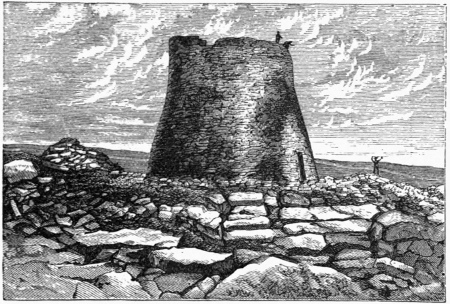
\includegraphics[width=\linewidth]{chast-colebanie-osnov/letois/fig160_197.jpg}
\textit{Broch of Mousa, Shetland.}
\end{center}

В статьях приводят замеры брохов – диаметр, высоту, но почему-то избегают сказать, какая была высота дверей. Но бывают и добросовестные ученые. Открываем книгу Джозефа Андерсона «Шотландия в поганские времена» («Scotland in pagan times», Joseph Anderson, 1881), по сути, сборник лекций. Лекция четвертая, «Устройство брохов». Рассматривается брох на острове Муса (Mousa), в Шетландии (архипелаг на северо-востоке Шотландии).

Про внешнюю дверь написано:

\begin{quotation}
Она на уровне земли, с юго-западной стороны, и около 5 футов 3 дюймов (1,524 метра) высотой и 2 фута 11 дюймов в ширину.
\end{quotation}

Далее идет описание, куда ведет тоннель от двери, то да сё, и потом описание внутренних помещений. Среди прочих там есть три комнатки, круглые, разной высоты – от 9 до 10 футов (2,7-3 метра), то есть можно не пригибаться, выше человека, но вот двери туда по три фута высотой и два в ширину, то есть 91 на 60 см. 

Существуют записки 17 века, шотландского священника городка Аберфойла, переводчика «Книги псалмов» на гаэльский, фольклориста Роберта Кирка (Robert Kirk), известные ныне под заголовком «The Secret Commonwe\-alth of Elves, Fauns and Fairies» («Тайное сообщество Элвов, Фаунов и Фэйри»).

Их предваряет описание:

\begin{quotation}
Природа и действия Подземного (и, в большей степени) Невидимого народа, известного под именем Элвов, Фаунов и Фэйри, или подобных, среди населения южной и восточной части Шотландии (Low-Country Scots), как они описаны теми, кто имеет Второе зрение; и теперь, для дальнейшего изучения, собранные и упорядоченные Осмотрительным исследователем среди Шотландско-Ирландского населения Шотландии. 
\end{quotation}

В этом небольшом произведении дается, с христианским оттенком, толкование необычных существ, способов их наблюдения, и взаимодействия с ними. Рассуждения, обобщения, многое размыто. Ощущаются недоговорки. По Кирку, фэйри или эльфы – отдельная раса, промежуточная между людьми и ангелами. У них тоже рождаются дети, бывают свои свадьбы и похороны. Среди них попадаются двойники людей из «нашего» мира.

Считается, что Кирк умер в 1692 году. И вот его преемник, священник Патрик Грэхем, в своем краеведческом путеводителе 1810 года «Sketches Descriptive of Picturesque Scenery, on the Southern Confines of Perthshi\-re», где немало места уделено фэйри, пишет, что Кирк вообще-то и не умер.

%Уолтер Скотт в своих «Письмах о демонологии и ведовстве» (Letters On Demonology And Witchcraft), изданных в первой половине 19 века пишет, со слов священника Патрика Грэхема из Абэрфойла

14 мая 1692 года, вечером, Роберт Кирк, отправился в одной ночной сорочке на так называемый Дан-ши, Doon Hill или холм Фэйри, небольшой пологий холм, что находился поблизости на запад от дома священника. Этот холм, поросший соснами и прочими деревьями, сейчас служит местной зловещей достопримечательностью.

На холме Роберт Кирк впал в состояние, которое сочли смертью, хотя, как замечает Вальтер Скотт в «Письмах о демонологии и ведовстве» (Letters On Demonology And Witchcraft), люди знающие могли бы определить в этом обморок, вызванный сверхъестественным влиянием народа, границы чьего владения он преступил. 

Роберта Кирка похоронили, однако после этого он неким образом явился, в той же ночной рубашке, одному из своих родственников и отправил того к Грэхему Дачрейскому (Duchray). Родич, с коему явился Кирк, тоже был родственником Грэхему Дачрейскому. Кирк поручил родичу следующее: «Иди к моему двоюродному брату Дачрэю и скажи ему, что я не мертв, я упал в обморок, и был перенесен в страну Фэйри, где теперь и нахожусь. Скажи ему, что когда он и мои друзья соберутся на крещении моего сына\footnote{Кирк оставил жену беременной.}, я появлюсь в помещении. Тогда, если Дачрэй бросит  над моей головой нож который он держит в руке, я буду освобожден и вернусь к обществу людей».

Родич однако не спешил передавать это сообщение. Тогда Кирк явился к нему повторно, угрожая преследовать его днем и ночью, если тот не передаст сообщение. Родственник наконец выполнил обещанное.

После церемонии крещения, все уселись за столом. Тут, якобы покойный, Роберт Кирк вошел в комнату через одну из дверей, но лорд Дачрэй по какой-то причине не бросил нож как было условлено. Роберт Кирк вышел через другую дверь и больше его не видели.

%, что смерть Кирка была необычной. Под вечер он вышел на прогулку по соседнему холму фэйри (dun-shi), и был найден в бессознательном состоянии, которое приняли за смерть. Преподобный Грэхем отметил, что знающие поняли бы, что это состояние вызвано сверхъестественным влиянием людей, чьи границы Кирк нарушил.

%После похорон, Кирк однако неким образом посетил родича, и попросил его передать на словах послание их общему двоюродному брату Грэхему из Дачрэя. Дескать, Кирк не мёртв, а пленен в стране Фэйри (Fairyland), и чтобы он смог вернуться, надо выполнить следующее. Жена Кирка осталась беременной. Когда она родит, Кирк будет при крещении младенца присутствовать в комнате. Тогда же брат должен бросить нож или кинжал поверх головы Кирка, и тот сможет вернуться к людям\footnote{Послание Кирка: «Say to Duchray, who is my cousin as well as your own, that I am not dead, but a captive in Fairyland, and only one chance remains for my liberation. When the posthumous child, of which my wife has been delivered since my disappearance, shall be brought to baptism, I will appear in the room, when, if Duchray shall throw over my head the knife or dirk which he holds in his hand, I may be restored to society; but if this opportunity is neglected, I am lost for ever.» – по Walter Scott, Letters On Demonology And Witchcraft.}.

%Кирк в самом деле появился на крещении, его видели, но Грэхем не выполнил просьбу, и Кирк лишился возможности вернуться.

Понятие «эльфов» и «фэйри» довольно размытое, отличается от местности к местности, и является общим названием, а не обозначением определенного вида существ. Можно сказать, что к эльфами относят сообщества перешедших в некий иной режим существования людей (и представителей других биологических видов) с особыми способностями, как Туаха де Дананн, а также просто некоторых умерших (подобное представление бытует у Славян в связи с русалками). Будучи в этом ином режиме существования, они изредка взаимодействуют с нами, обычно в особых местах и условиях.

%Например, Исландцы делили своих «альвов» на черных (подземных) и светлых (живут в Алфхэйме). Бытовало и мнение о трех видах, выраженное Йоуном Гвюдмундссоном Ученым (Jón lærði Guðmundsson, 1574-1658) в рукописи «Собрание сведений и фактов для лучшего понимания Эдды» (1641)\cite{korabl01}: 

%\begin{quotation}
%Люди полагают также, что эльфы – это народ, делящийся на три рода, или имеющий три основных места обитания. Одно – в море. Второе – внутри земли или под землей, которое люди называют «Эльфо-мир», а иногда – подземный мир, что многие наши истории поясняют. И люди видят, что этот род не имеет носового хряща между ноздрями. Живут же они половину обычного нашего срока (на земле). Третий род, который мы называем Сокрытым Народом или льювлингами также населяет холмы и скалы; и часто сочетались они с нашим родом. Этот эльфийский род живет дольше, отличается красотой и имеет правильную форму, как у нас.
%\end{quotation}

С эльфами связано иное течение времени. Это проявляется в следующих случаях. Ребенок, рожденный от эльфов (чистый эльф или полукровка) растет быстрее (среди людей), нежели дитя человеческое.

Живые люди, попадавшие в мир эльфов (осознаю всю условность этого определения), возвращались в мир людей спустя долгие годы, при этом для них прошло совсем немного времени. Значит, в мире эльфов время течет медленнее, чем в нашем. Однако возвращаясь оттуда, некоторые люди быстро старели, едва не на глазах. 

Любопытно, что мы знаем еще один мир с иным течением времени – мир снов, в котором время течет быстрее нашего. Таким образом выстраивается цепочка «миров», различных по скорости времени. Расположу по возрастающей: мир эльфов → мир людей → мир снов.

Какое всё это имеет отношение к Киеву? А я непроста рассказываю, позже всплывет.

Некоторые из героев ирландских анналов и сказаний, например Луг, были обожествлены, стали языческими богами. Выдающаяся личность сегодня, через век ее почитают за божество, а спустя еще пару столетий, когда переменяется вера – уже называют демоном. 

Ирландским анналам повезло, их не сократили под корень, оставили ирландцам прошлое. Наши же летописи, относящиеся к Киеву, словно отрублены на уровне князя Кия. И кто знает, повествование о каких событиях мы бы прочитали за предшествующие годы, и какие бы люди – или нелюди – действовали в них?

Но заглянуть за эту черту таки возможно, ведь кроме летописей, существуют и другие, внешние источники.
